\documentclass[14pt]{article}
\usepackage{amsmath}
\usepackage{listings} % For writing code see http://ctan.org/pkg/listings
\usepackage{graphicx}
\usepackage{float}
\usepackage[margin=1.0in]{geometry}
\usepackage{hyperref}

\title{Dynamical model of NGC2419}
\author{Nicolas Garavito-Camargo}
\begin{document}
\maketitle


In this document different dynamical models of \textbf{NGC2419} are explored
in the presence of the Sagittarius dwarf galaxy (Sgr) and the Large
Magellanic cloud (LMC). The document is structured as follows, in section
\ref{sec:test} the code to compute the orbits is tested with the
public available code \textsc{GalPy}, in section \ref{sec:NGC} the
orbits of NGC2419 are integrating around a spherical MW potential,
in section \ref{sec:NGCSgr} orbits of NGC2419 are integrated in a
spherical MW potential and including the presence of Sgr.
 In the las section the orbit of NGC2419 are integrating
with both the presence of Sgr and the LMC.

\section{Testing the code:}\label{sec:test}

A test particle integrated in a NFW profile both with \textsc{Galpy}
and the code developed for this work.

\begin{figure}[H]
\centering
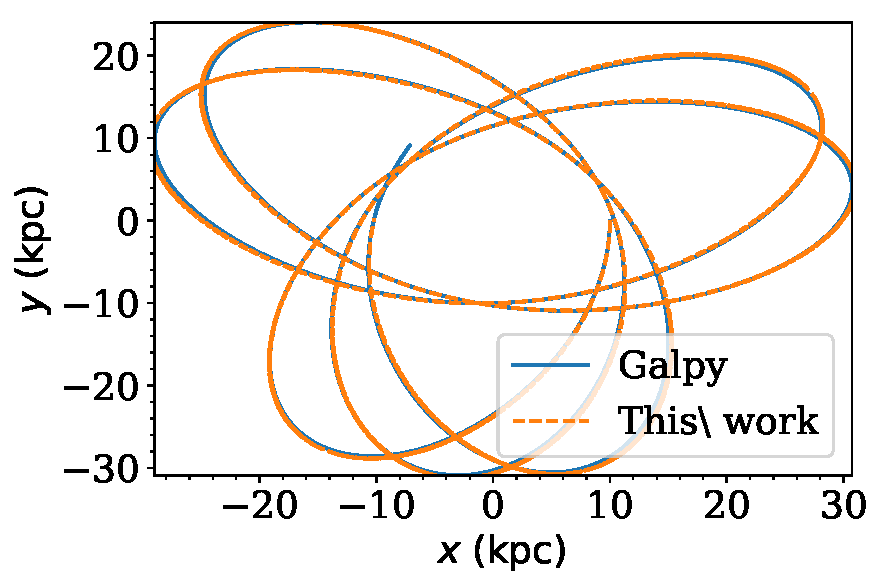
\includegraphics[scale=0.5]{../exploratory_code/galpy_test.pdf}
\end{figure}


\section{The orbit of NGC2419 around the MW}\label{sec:NGC}

Table 1 summarizes the MW models used in the following orbit analyzes.

\begin{table}[H]
\centering
\begin{tabular}{c c c c c}
\hline
\hline
\textbf{Models:} & & & & \\
\hline
\textbf{Model 1:} & & & & \\
Halo: & NFW & $M_{vir} = 1\times 10^{12} M_{\odot}$ & $c=9.86$  \\
Disk: & Miyamoto-Nagai & $M_{d} = 6.5\times10^{10} M_{\odot}$ & $r_L = 3.5 kpc$ & $r_H = 0.53 kpc$ \\
Bulge: & Hernquist & $M_b = 1 \times 10^{10} M_{\odot}$ & $r_s=0.7 kpc$ & \\
\hline
\textbf{Model 2:} & & & & \\
Halo: & NFW & $M_{vir} = 1.5\times 10^{12} M_{\odot}$ & $c=9.56$  \\
Disk: & Miyamoto-Nagai & $M_{d} = 6.5\times10^{10} M_{\odot}$ & $r_L = 3.5 kpc$ & $r_H = 0.53 kpc$ \\
Bulge: & Hernquist & $M_b = 1 \times 10^{10} M_{\odot}$ & $r_s=0.7 kpc$ & \\
\hline
\textbf{Model 3:} & & & & \\
Halo: & Triaxial NFW & $M_{vir} = 1.45\times 10^{12} M_{\odot}$ &
$c=20$  & $q=0.8$, $s=1$. \\
Disk: & Miyamoto-Nagai & $M_{d} = 4\times10^{10} M_{\odot}$ & $r_L = 3.5 kpc$ & $r_H = 0.53 kpc$ \\
Bulge: & Hernquist & $M_b = 1 \times 10^{10} M_{\odot}$ & $r_s=0.7 kpc$ & \\
\hline
\hline
\end{tabular}
\caption{Milky Way model parameters}
\end{table}

I'm assuming $q=b/a$, $s=c/a$, $a>b>c$, \textit{In Massari+17 they
mention that $q=0.8$ , but in Hayashi07 they use c/a=0.8 therfore I
think there is a notation problem regardin weather q=0.8 or s=0.8 }


\begin{figure}[H]
\centering
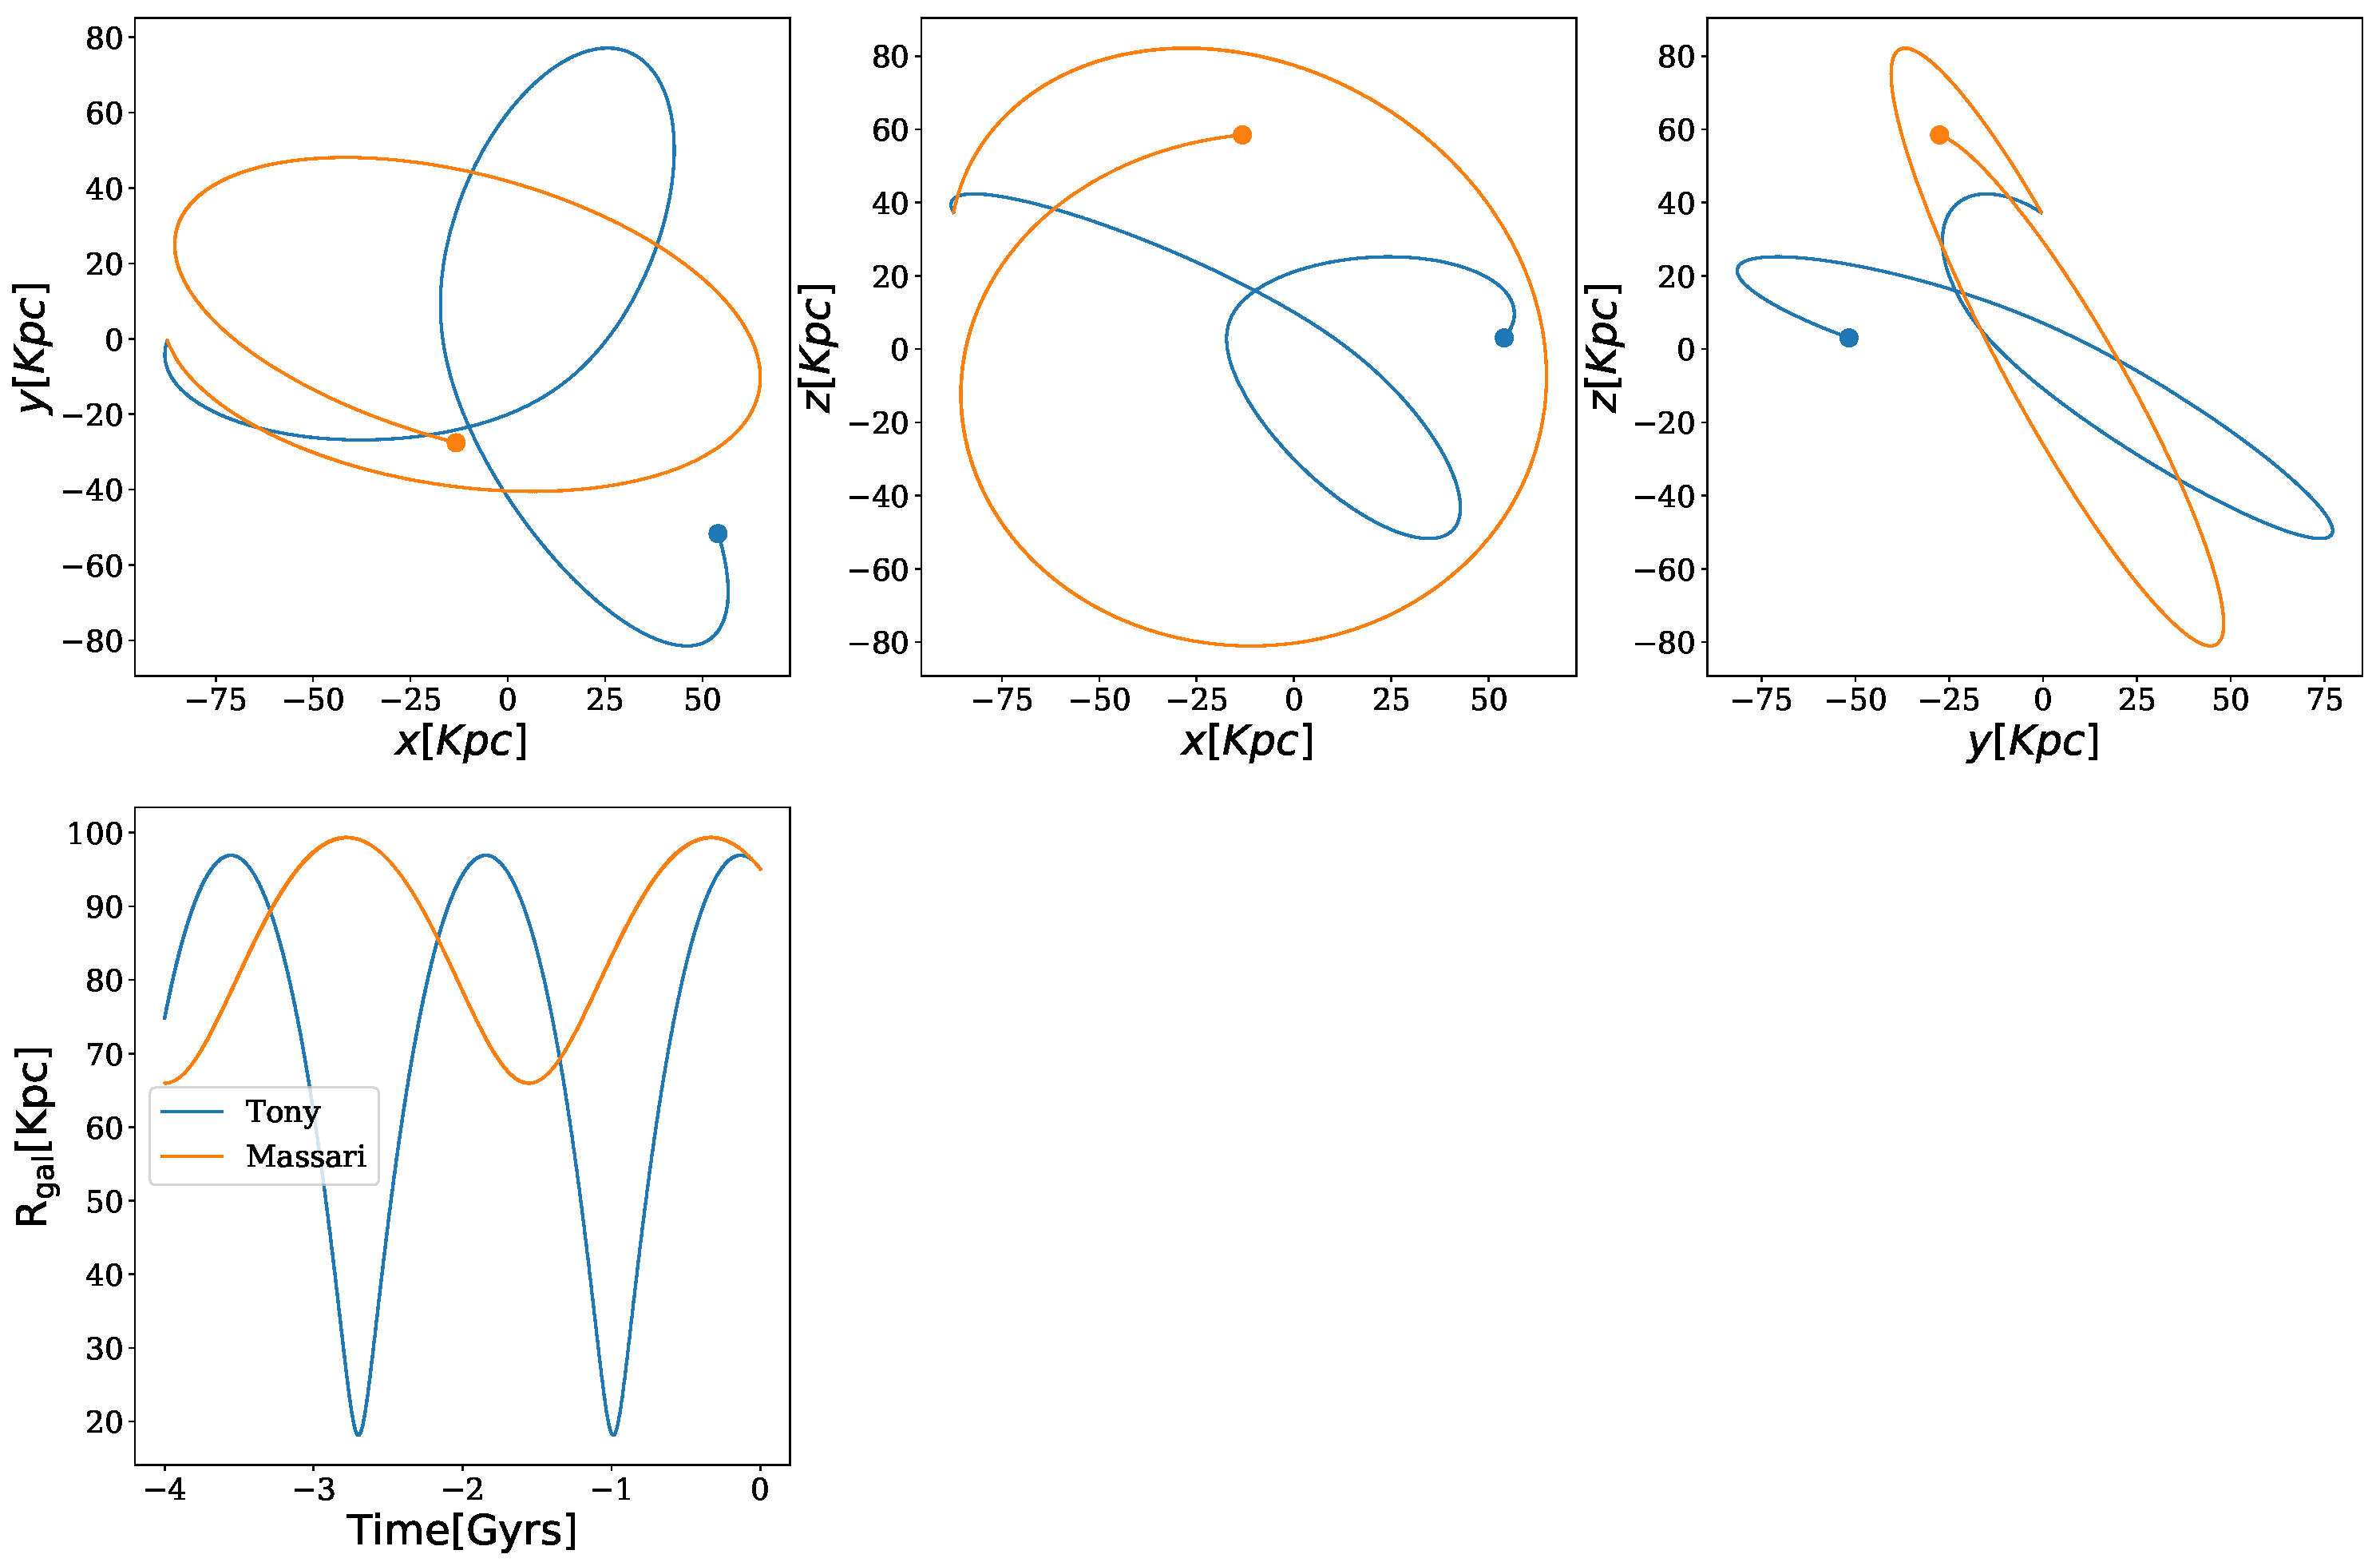
\includegraphics[scale=0.3]{../exploratory_code/NGC2419_sphMW.pdf}
\caption{Orbits of NGC2419 using Model 1, blue line correspond to
the orbit using Tonys proper motions measurements while the orange line correspond to
Massari16 proper motion.}
\end{figure}

The angle between this orbits is $35.7^{\circ}$ this is best seen in
\href{https://plot.ly/~jngc/3/orbits/?share_key=FcyuVOnd0LYVXaYhGmSuo9}{this}
3D visualization. This plot also showis easily seen that the plane of the orbit for the two
different proper motions are very different.

\begin{figure}[H]
\centering
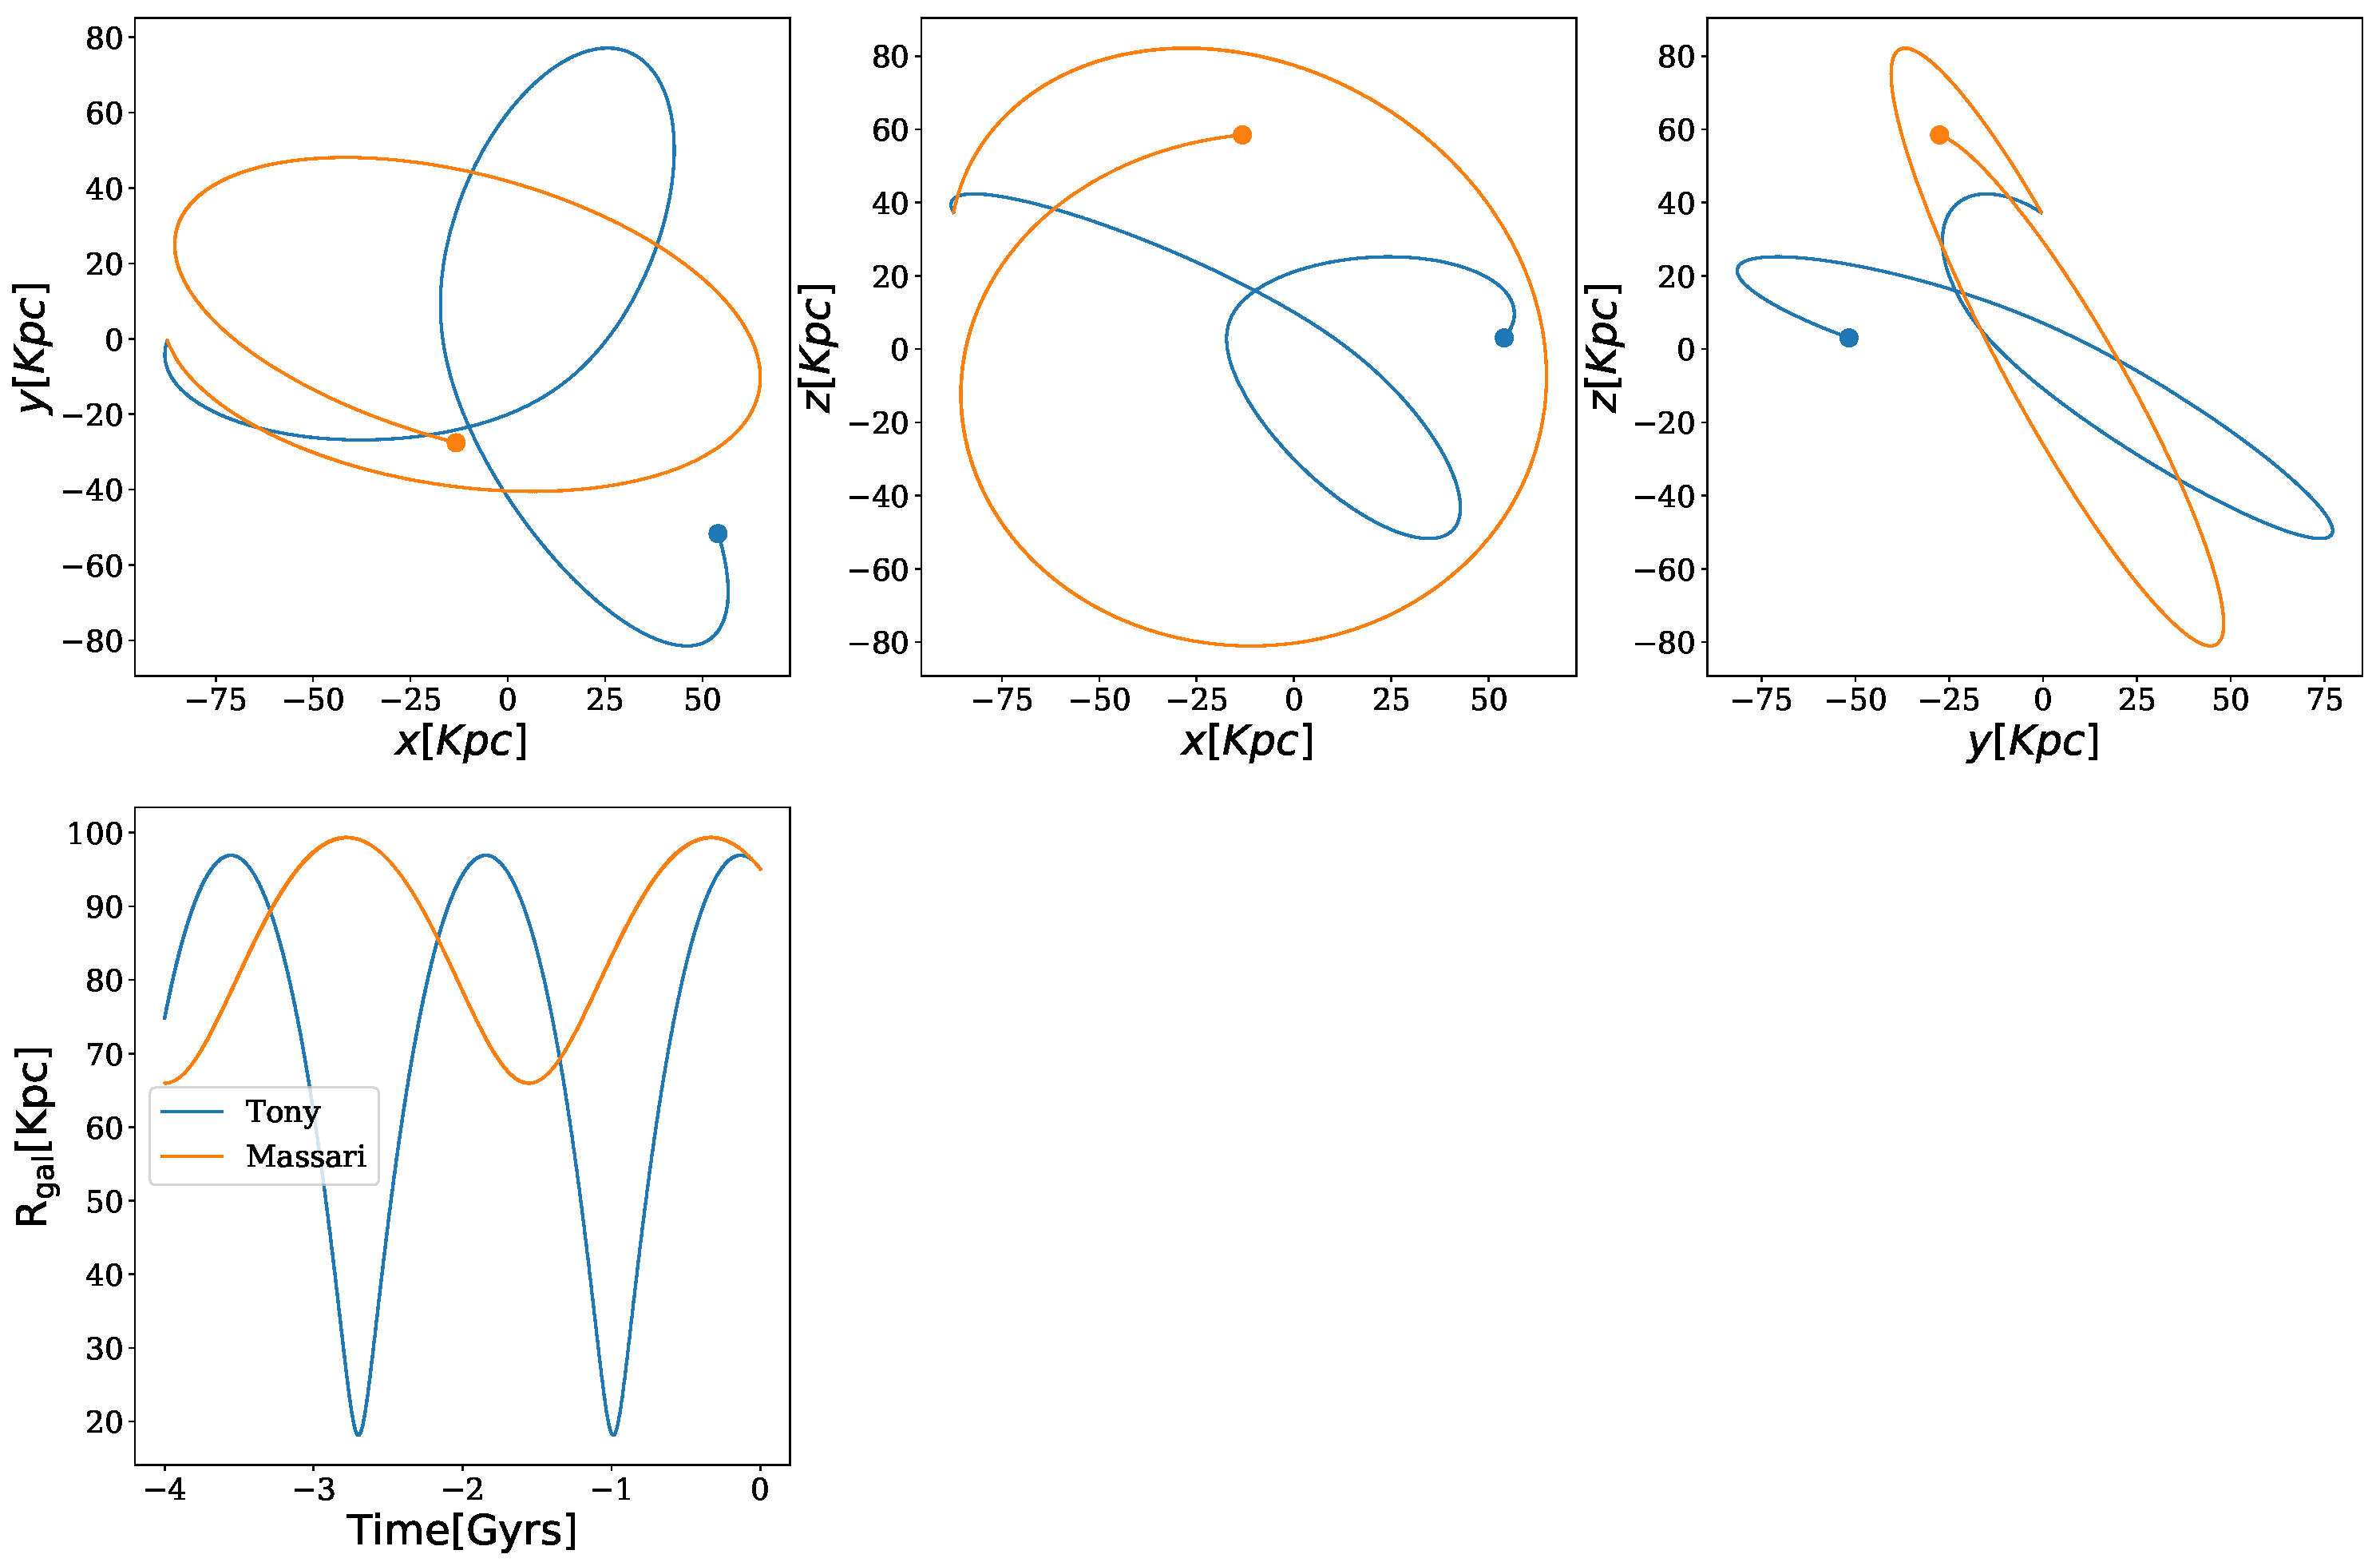
\includegraphics[scale=0.3]{../exploratory_code/NGC2419_sphMW.pdf}
\caption{Orbits of NGC2419 using Model 2, blue line correspond to
the orbit using Tonys proper motions measurements while the orange line correspond to
Massari16 proper motion.\label{fig:model2MW}}
\end{figure}

Figure \ref{fig:model2MW} shows how the period of the orbit decreases
with increasing the halo mass, in particular for the orbit with the
new proper motions.


\begin{figure}[H]
\centering
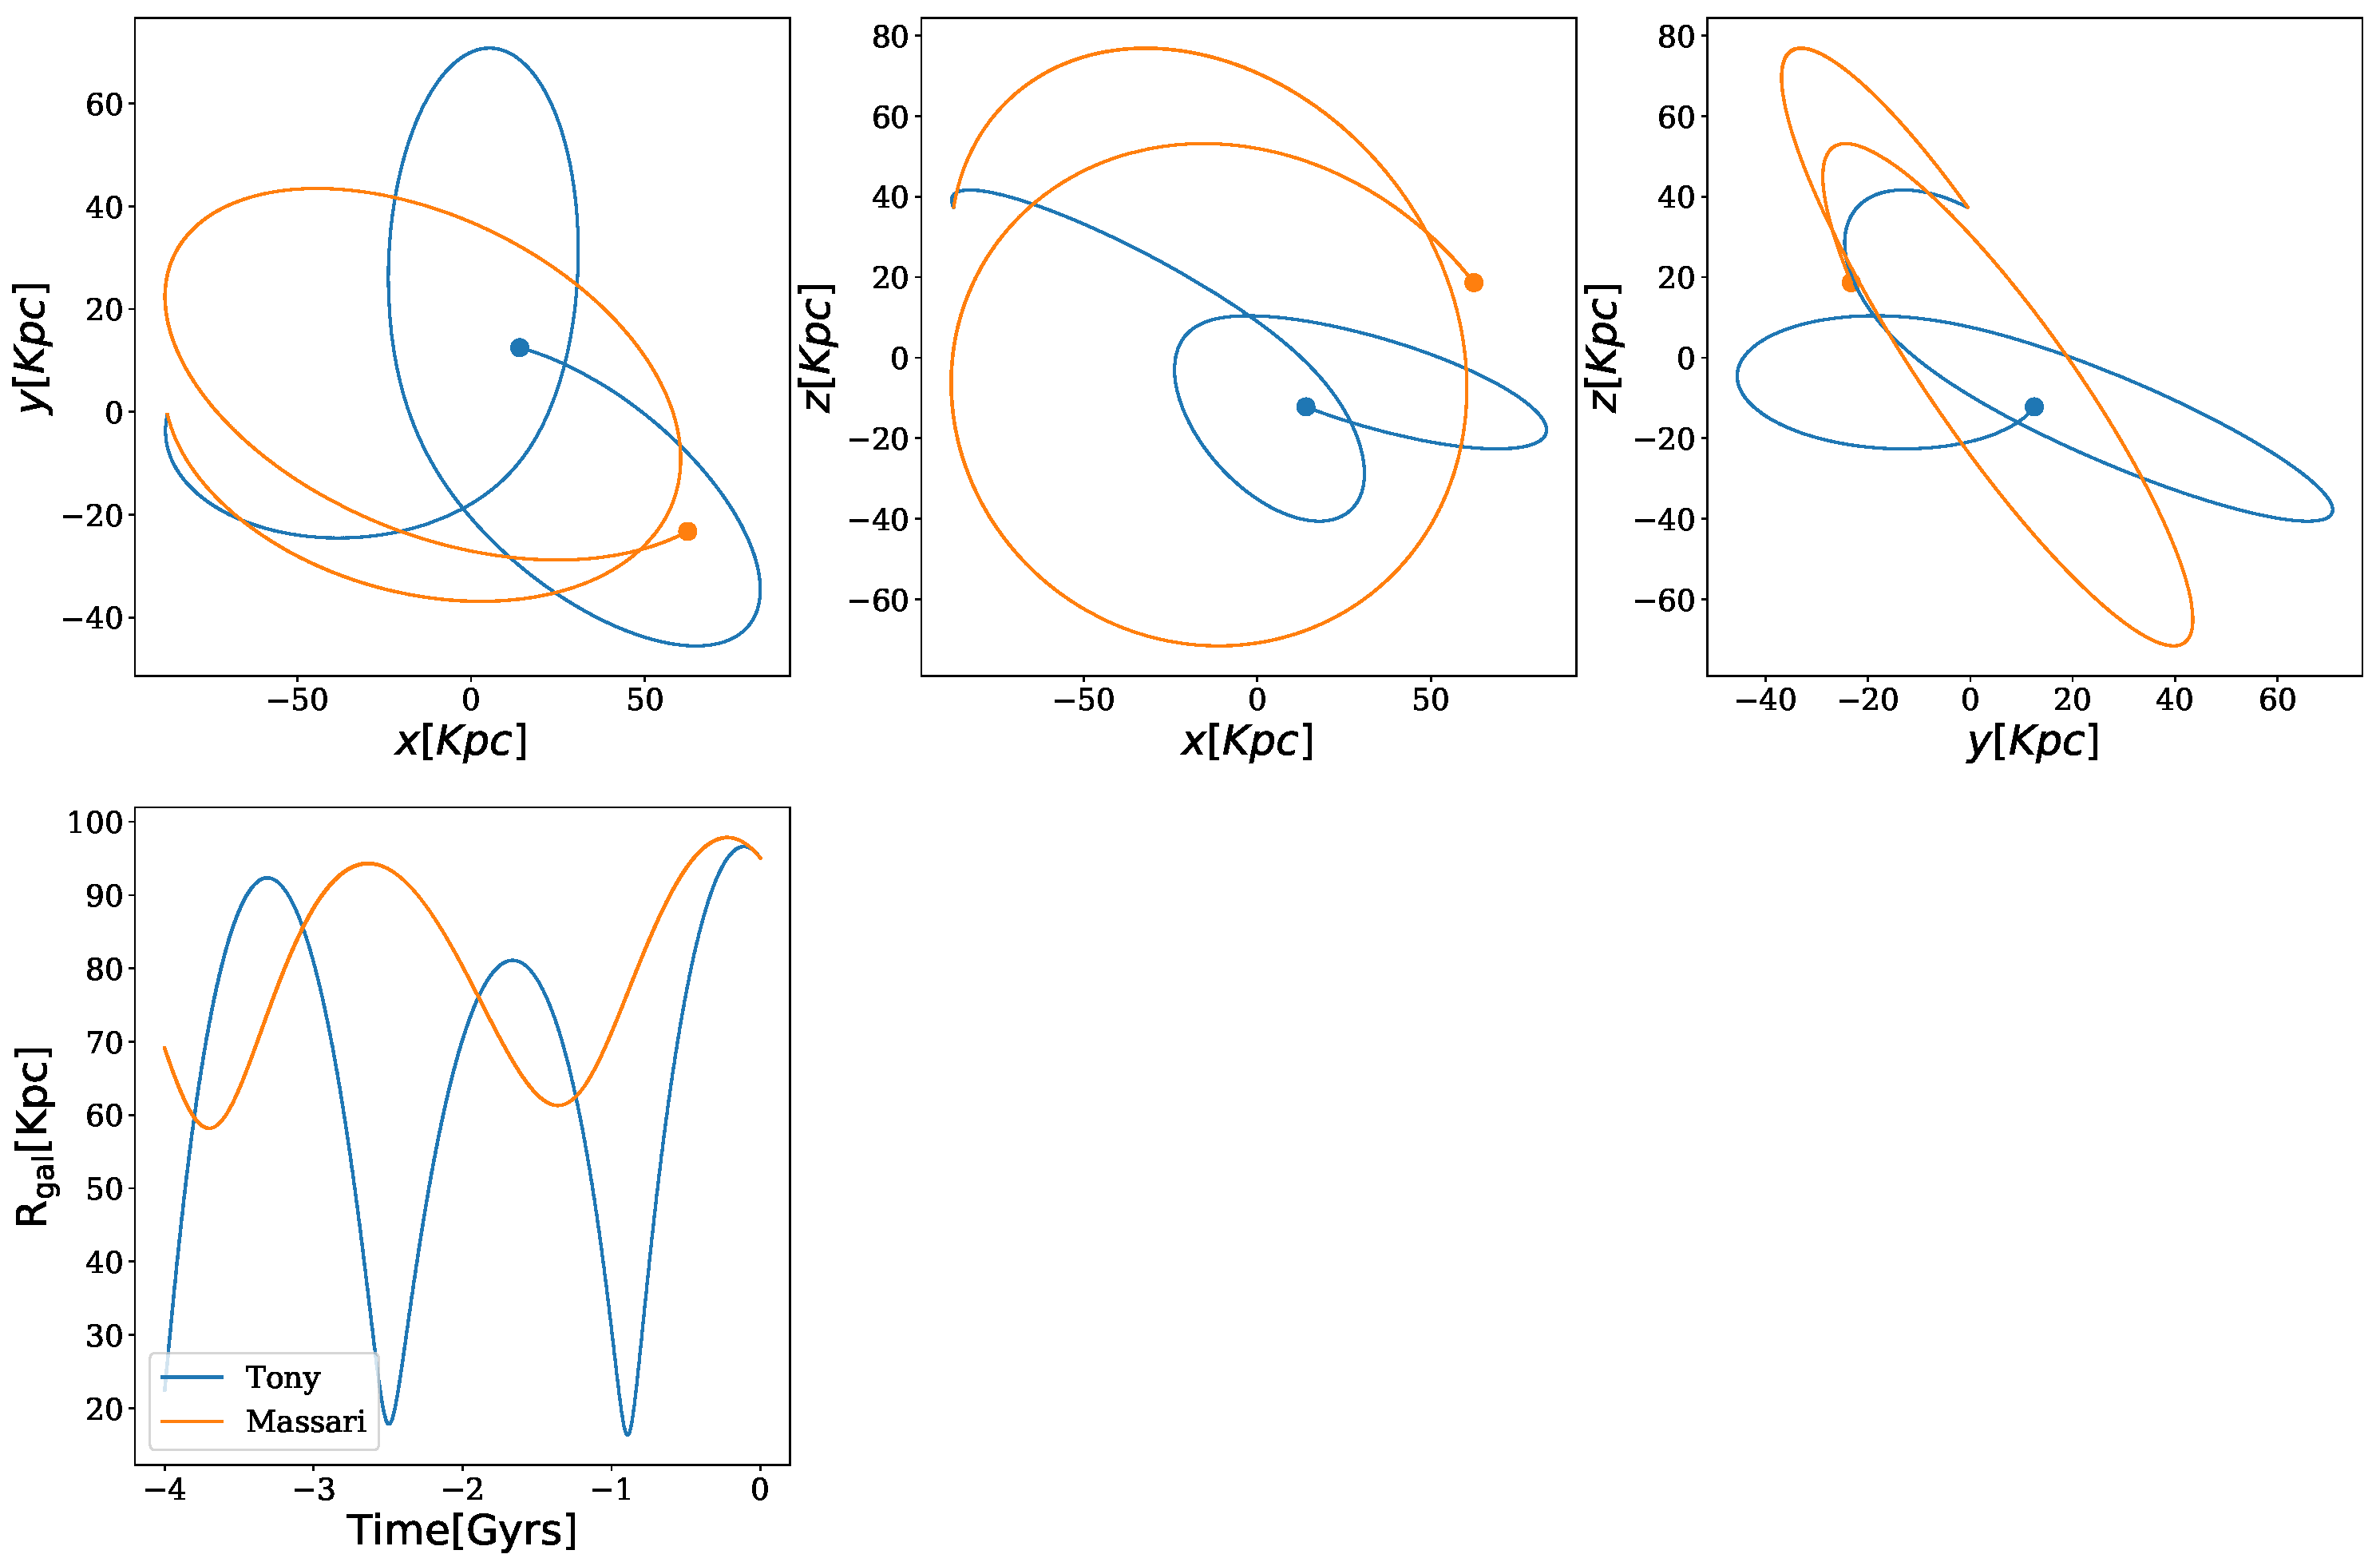
\includegraphics[scale=0.3]{../exploratory_code/NGC2419_Triaxial_MW.pdf}
\caption{Orbits of NGC2419 using model 3. This is the MW model used by
Massari et al 2016.}
\end{figure}



\section{The orbit of NGC2419 around the MW with Sgr}

In this section we include the effect of the Sagittarius (Sgr) dwarf
galaxy, to this aim we integrate the orbit from the present time. In
this 3-body interaction the MW is free to move due to the
gravitational interaction with Sgr. NGC 2419 feels both the force
from the MW and Sgr. To model the orbit of Sgr we include the dynamic
friction effect by implementing the Chandrasekhar equation, the
Coulomb Logarithm is modified following a similar procedure as the one
in Van Der Marel (XX) in order to account for extended satellites in 
order to reproduce the orbit of Sag from N-body simulations such as 
Diercxx. The model used to represent Sgr is summarized in table
\ref{tab:Sgrmodel}.


\begin{table}[H]
\centering
\begin{tabular}{c c c c c}
\hline
\hline
Halo: & NFW & $M_{vir} = 1\times 10^{10} M_{\odot}$ & $c=8$  \\
\hline
\hline
\end{tabular}
\caption{Sagittarius dwarf model.\label{tab:Sgrmodel}}
\end{table}


Figure \ref{fig:Sgrmodel1} shows the orbit of NGC2419 (Organge) in the
presence of Sgr (Blue), the orbit of NGC2419 using the old proper
motion measurement is shown in green, the blue line shows the tidal
radius of Sgr $r_t = r_{peri} (M_{sat}/(2*M_{MW(r_{peri})}))^{1/3}$.
The angle between the orbits of NGC2419 and Sgr is $55.59$ while the
angle between the plane of the orbit for the old NGC2419  and Sgr is
$24.68$.

\begin{figure}[H]
\centering
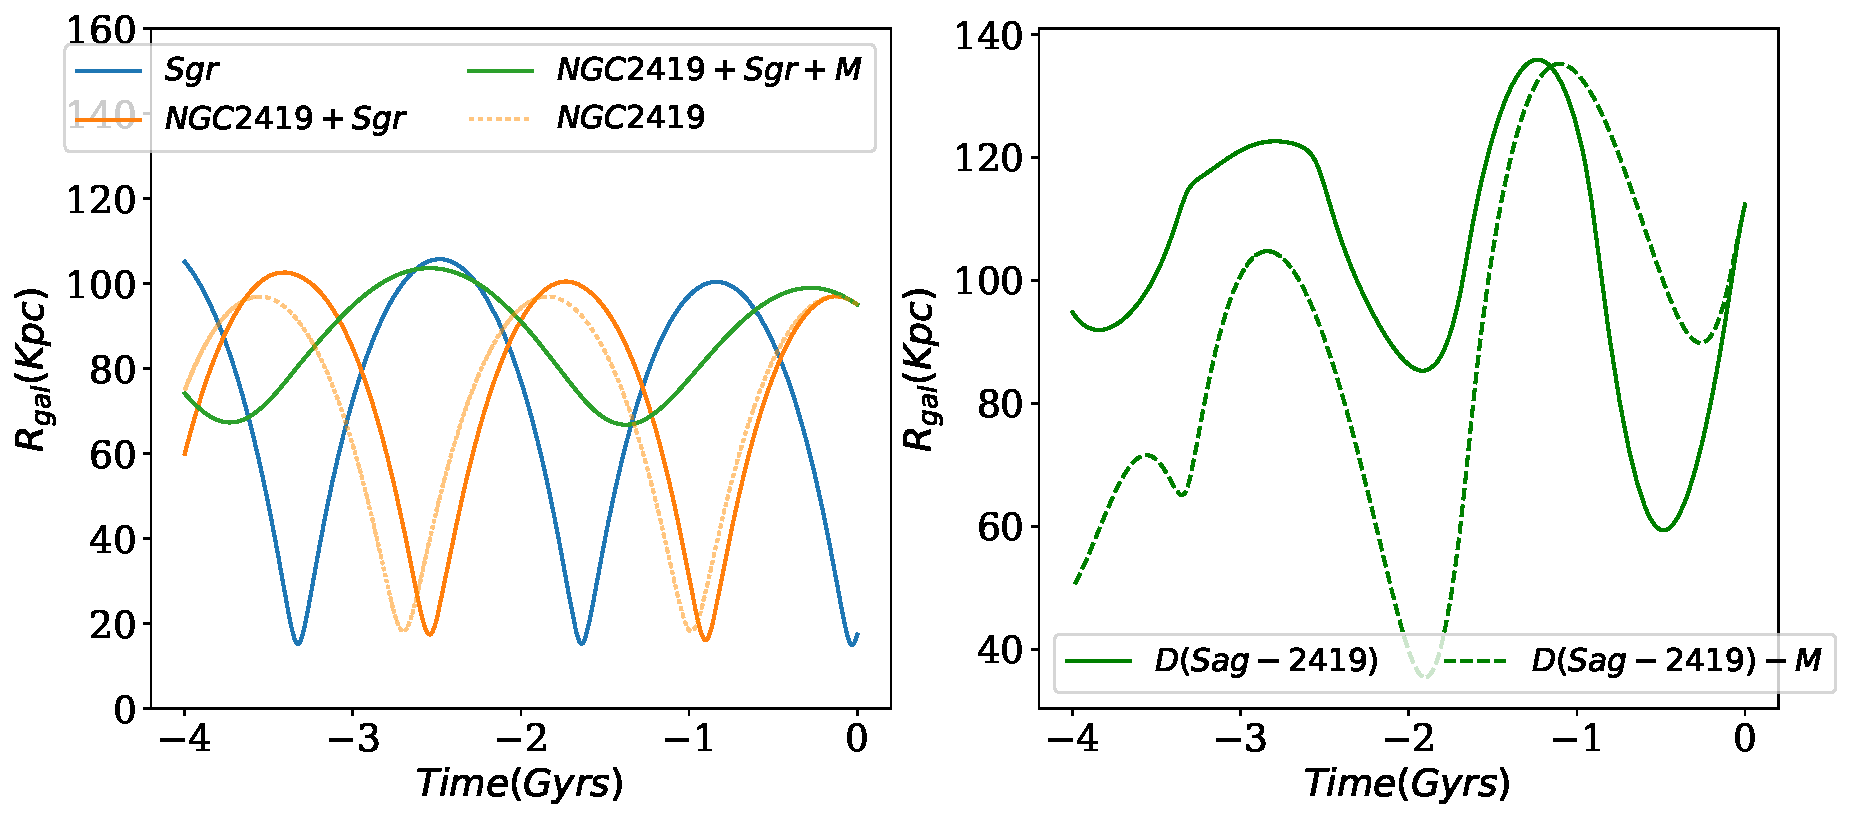
\includegraphics[scale=0.5]{../exploratory_code/NGC2419_sphMWSGR.pdf}
\caption{Right: Orbits of NGC2419 (orange), Sgr (blue), and NGC2419
with Massari+17 proper motion. Left: Distance between NGC2419 and Sgr
as function of time for the new (solid line) and old proper motion
(dashed). \label{fig:Sgrmodel1}}
\end{figure}

A 3D visualization of this plots can be found \href{https://plot.ly/~jngc/22/orbits/}{here}

Figure \ref{fig:Sgrmodel2} the same as in figure \ref{fig:Sgrmodel1}
but using model 2.

\begin{figure}[H]
\centering
\includegraphics[scale=0.5]{../exploratory_code/NGC2419_sphMWhSGR.pdf}
\caption{\label{fig:Sgrmmodel2}}
\end{figure}

The orbit of Sgr in model 1 and in model 2 is in the same plane.
\href{https://plot.ly/~jngc/25/orbits/}{here}



\section{The orbit of NGC2419 around the MW with Sgr and the LMC}

LMC masses: $[3\times10^{10}, 5\times10^{10}, 8\times10^{10},
1\times10^{10}, 1.8\times10^{11}, 2.5\times10^{11}]$



\begin{figure}[H]
\centering
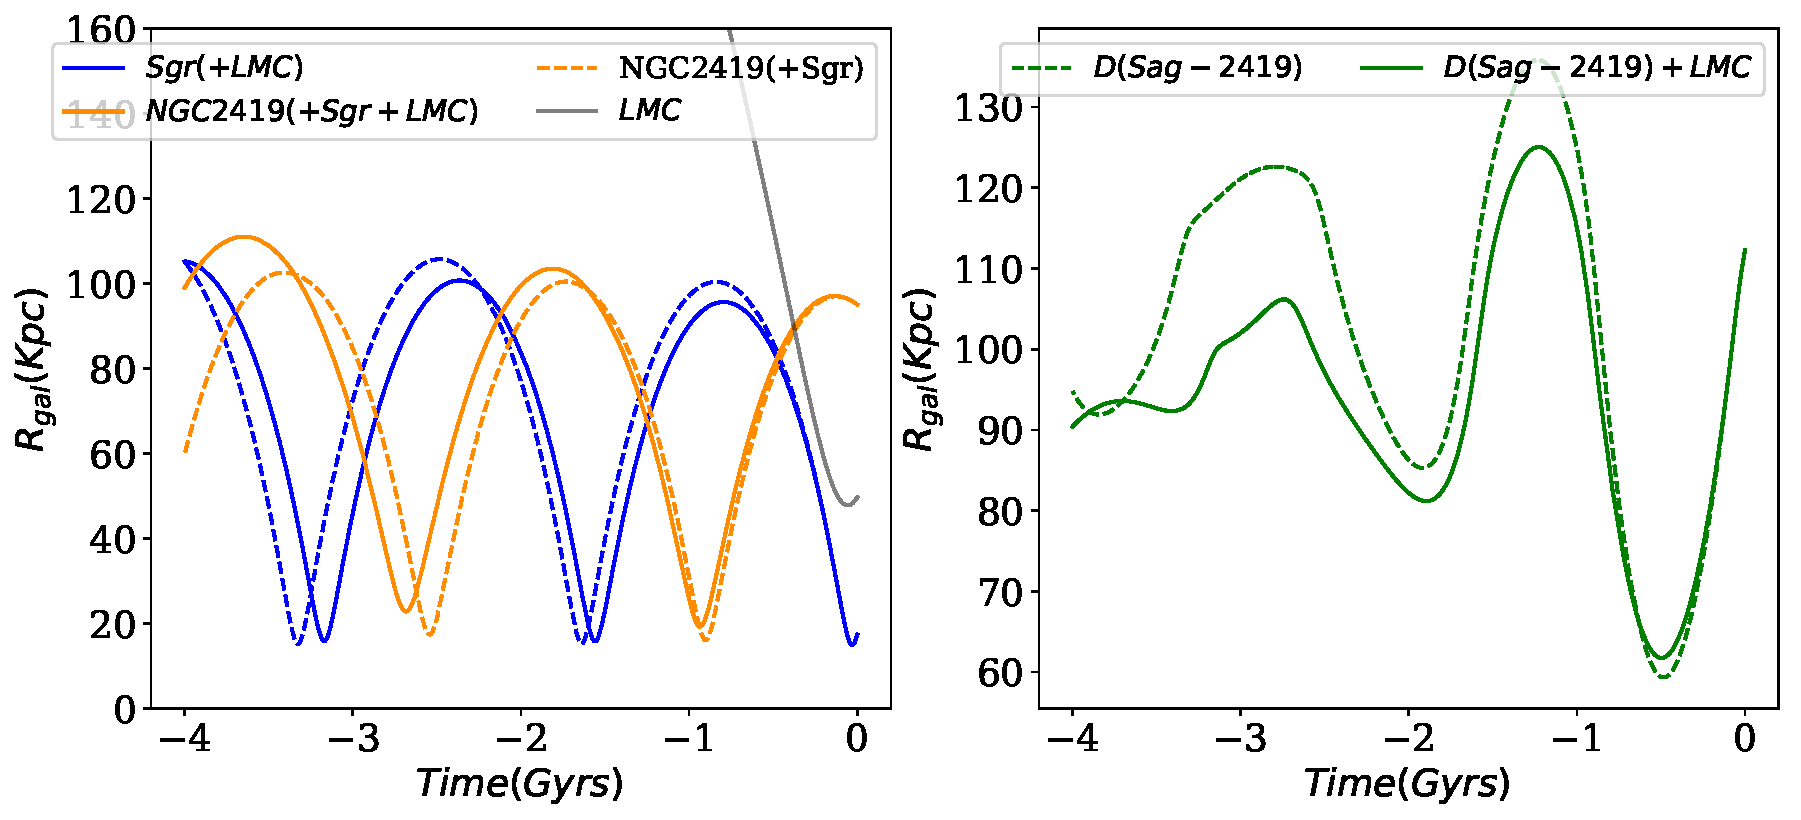
\includegraphics[scale=0.5]{../exploratory_code/NGC2419_sphMWSGRLMC.pdf}
\caption{For the lightest LMC and lightest Sag.}
\end{figure}


\begin{figure}[H]
\centering
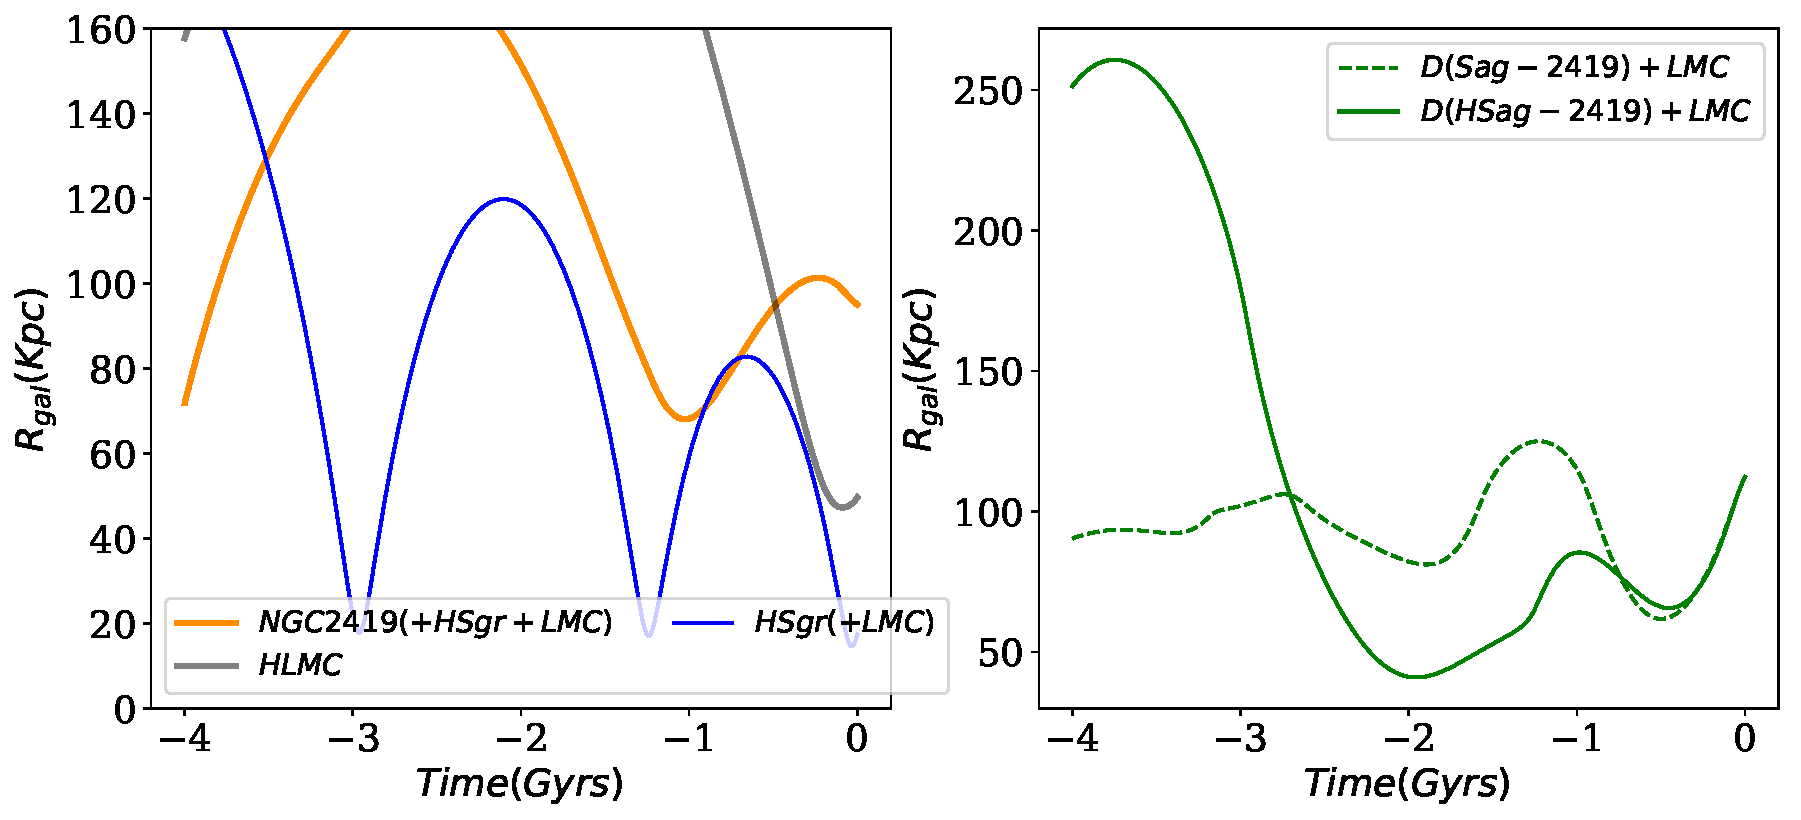
\includegraphics[scale=0.5]{../exploratory_code/NGC2419_sphMWHSGRLMC.pdf}
\caption{for the lightest LMC and Heavy Sag.}
\end{figure}

\begin{figure}[H]
\centering
\begin{minipage}{0.49\linewidth}
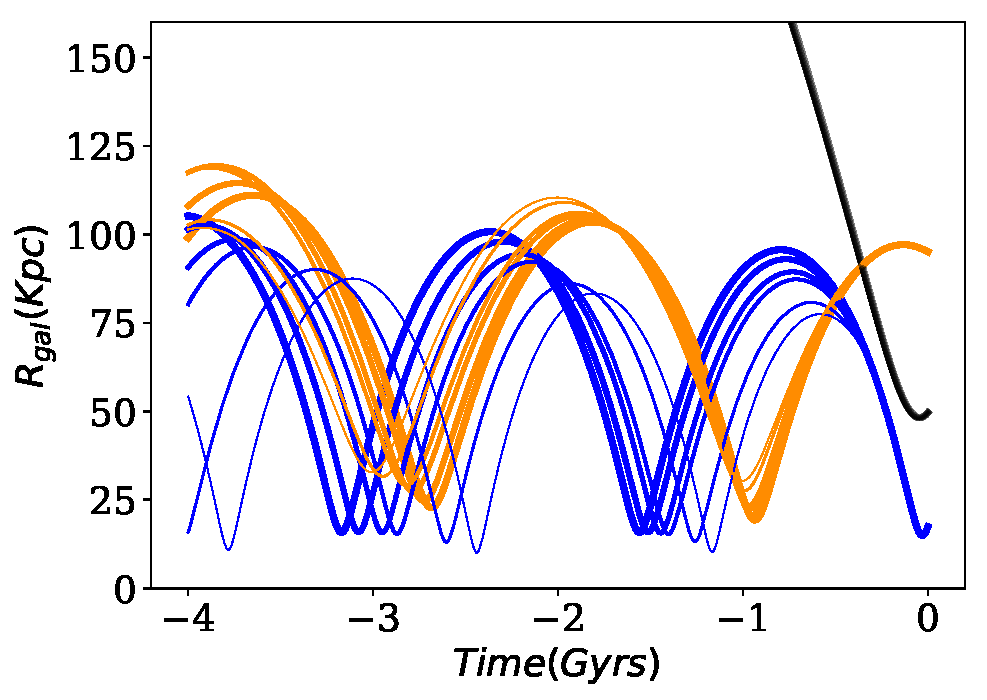
\includegraphics[scale=0.5]{../exploratory_code/gal_orbits_all_LMCs.pdf}
\end{minipage}
\begin{minipage}{0.45\linewidth}
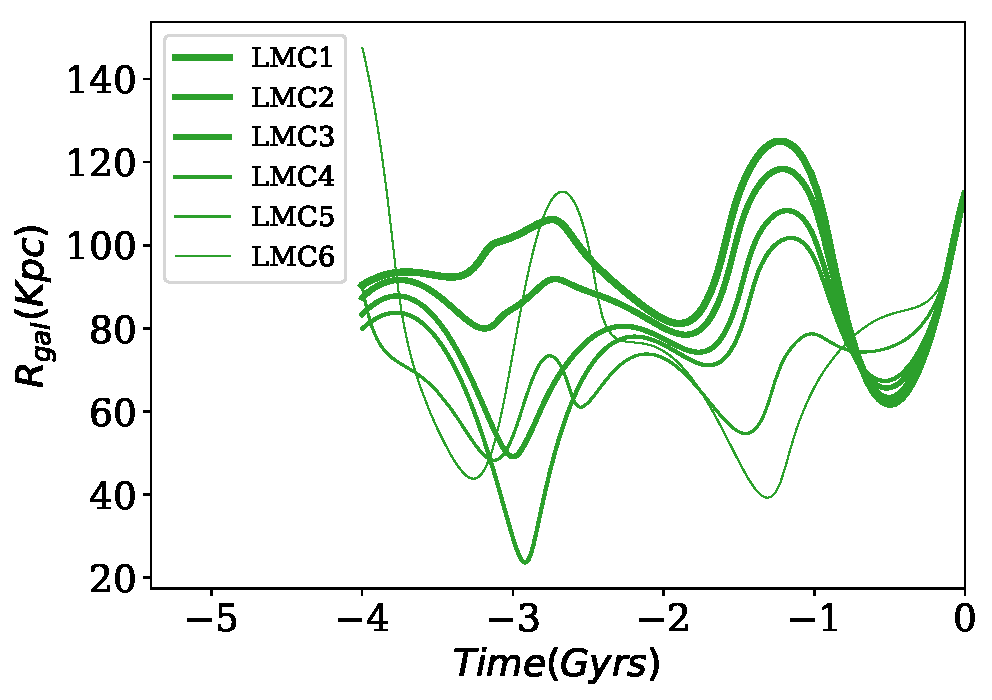
\includegraphics[scale=0.5]{../exploratory_code/d_rel_all_LMCs.pdf}
\end{minipage}
\end{figure}




\begin{figure}[H]
\centering
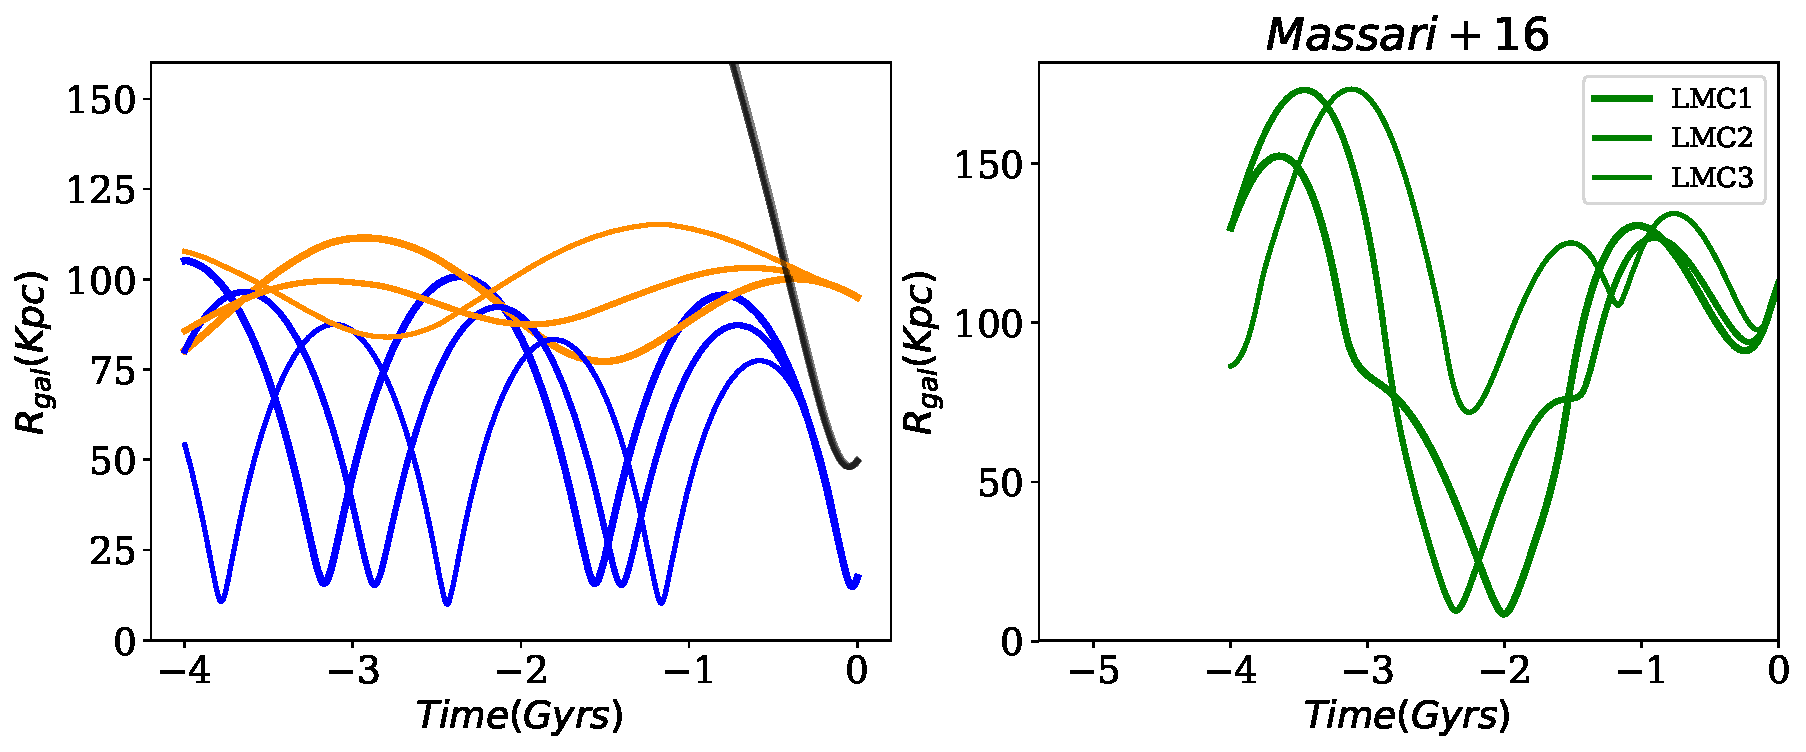
\includegraphics[scale=0.5]{../exploratory_code/gal_orbits_all_LMCs_massari.pdf}
\caption{NGC2419 IC taken from Massari+16 proper motion.}
\end{figure}

\section{The orbit of NGC2419 around the MW in a NFW triaxial
potential with the LMC}


The new potential is a NFW with $c=20$, $q=0.8$ and $s=1$ following
Massari+16.

\begin{figure}[H]
\centering
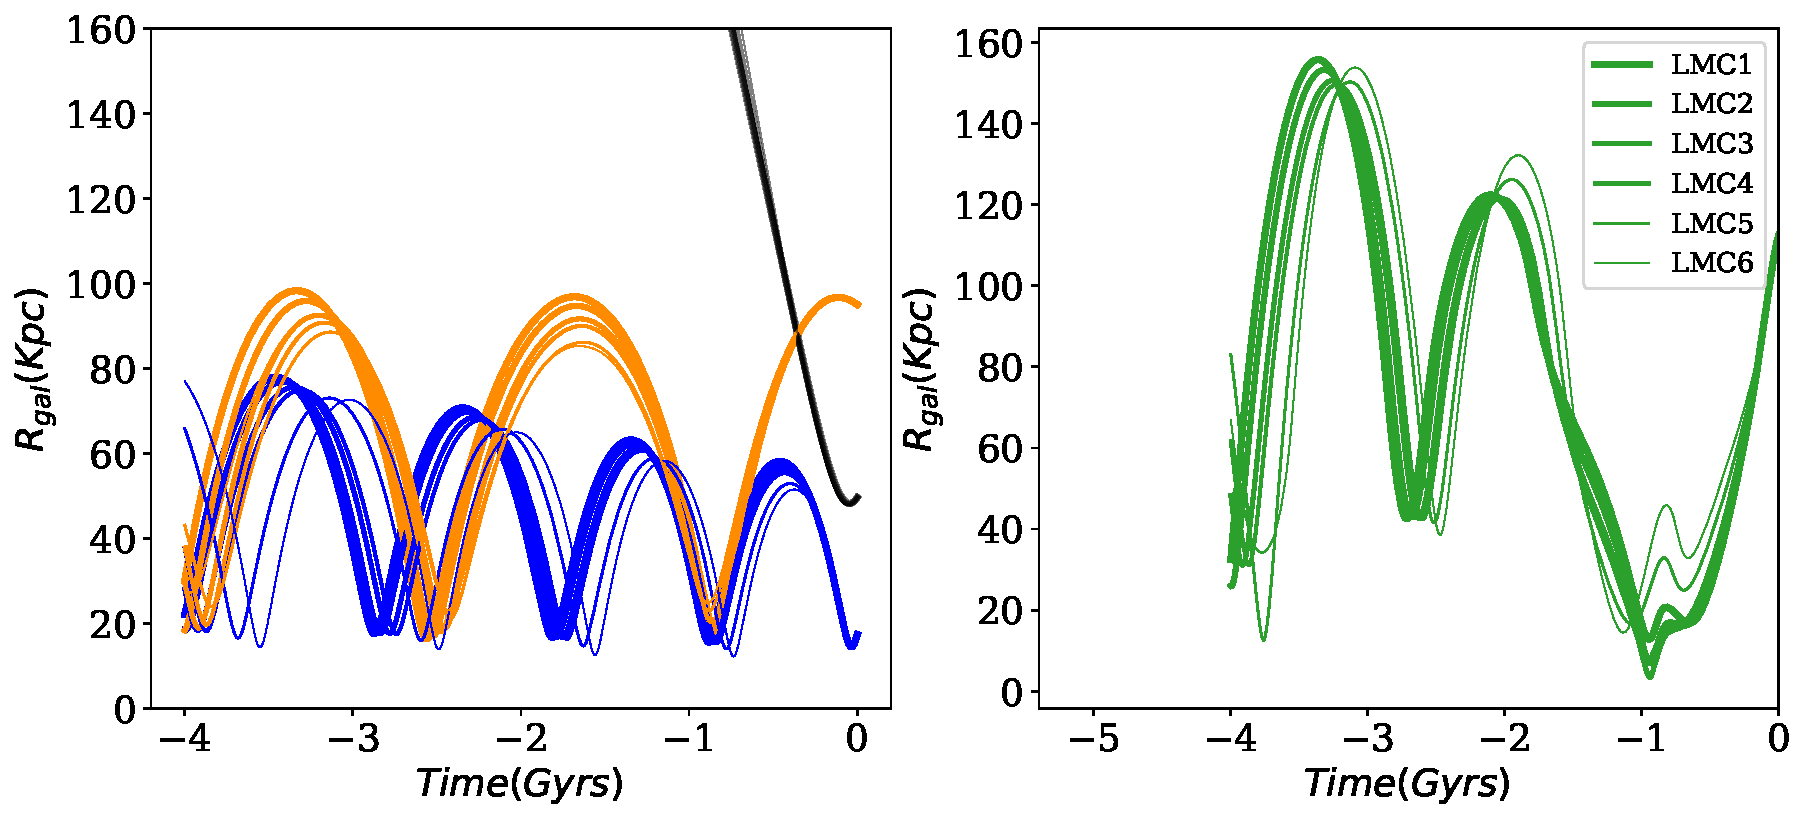
\includegraphics[scale=0.5]{../exploratory_code/gal_orbits_all_LMCs_Triaxial.pdf}
On the right panel the thickness of the line represent a higher mass
LMC
\end{figure}

\begin{figure}[H]
\centering
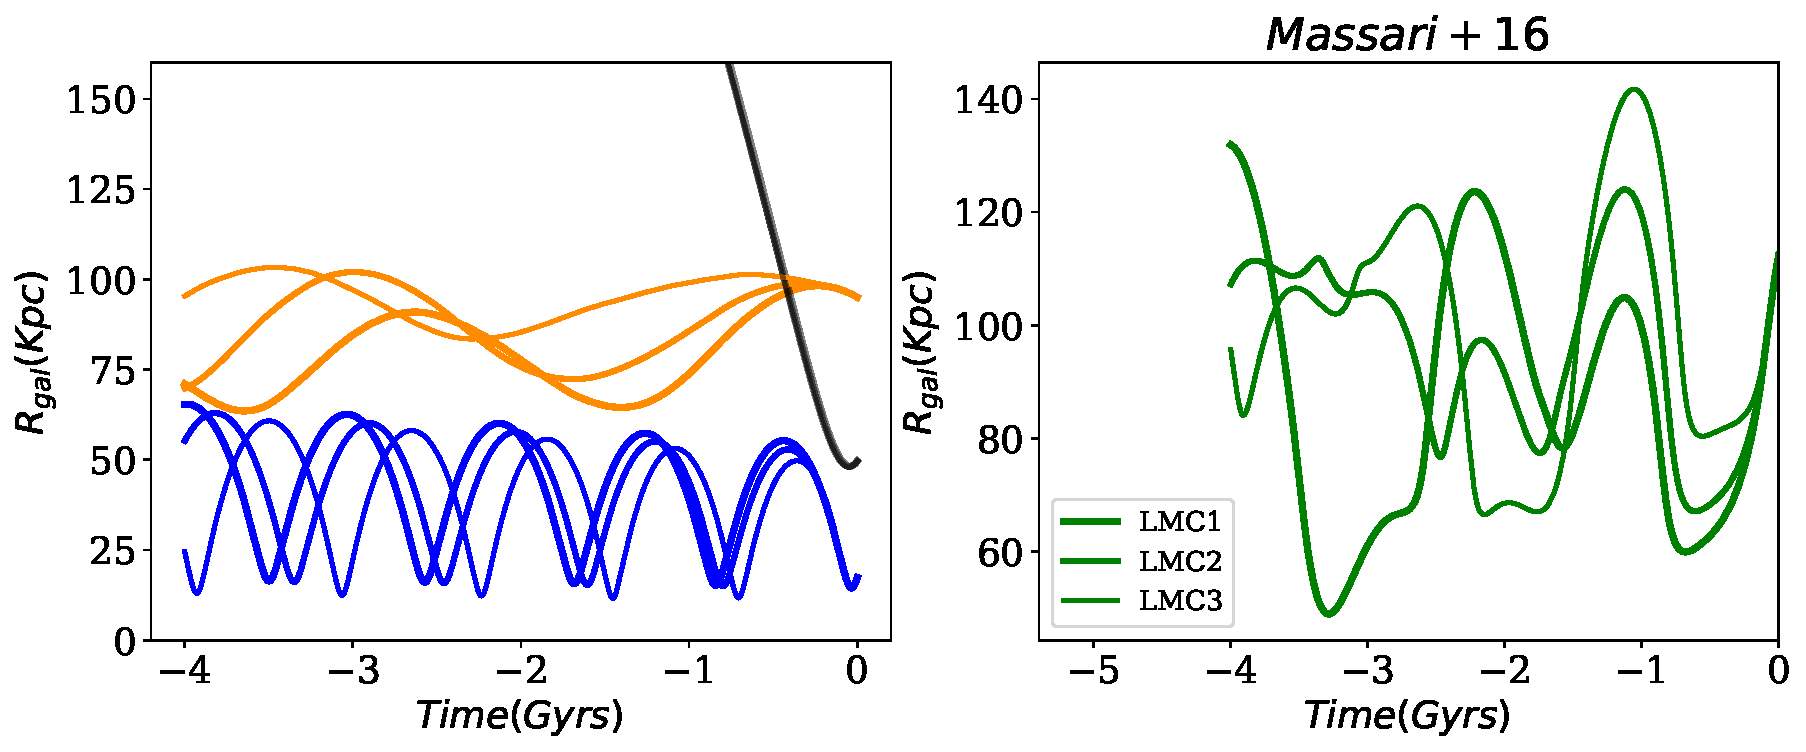
\includegraphics[scale=0.5]{../exploratory_code/gal_orbits_all_LMCs_massari_T.pdf}
\caption{NGC2419 IC taken from Massari+16 proper motion.}
\end{figure}

\end{document}

